\documentclass[10pt,a4paper]{article}
\usepackage[utf8]{inputenc}
\usepackage{amsmath}
\usepackage{amsfonts}
\usepackage{amssymb}
\usepackage{graphicx}
\usepackage{wrapfig}
\author{Flip van Spaendonck \& Lars Kuijpers \\ s4343123 \& s4356314}
\title{Compiler Construction Final Report}

\begin{document}
\maketitle
\tableofcontents

\section{Introduction}
\subsection{Programming language}
%programming language + motivation
\subsection{Error Handling}
%error handling (code shitty, expression shitty, type shitty, not yet declaration shitty)
\subsection{Final Grammar}
%final grammar


\section{Lexer}
\subsection{Basic structure}
Our lexer is based on the work shown in one of the practical sessions and made available on Blackboard. We've continued the work done there to include all inputs necessary to tokenize the SPL language (and our extensions). \\
\\
Our lexer accepts a string as an input, which will be saved locally. The lexer can then be asked for either the next token, or all next tokens with two seperate functions. With the nextToken() function, the lexer will skip any whitespace that is on its current position, until it finds another character. Depending on which character it finds, the function will return a specific token corresponding with that character. Sometimes determining which token to return requires looking at more than a single character, in which case the function will look at the next character in the input as well. If the next character is one of the expected ones, the function will return the corresponding token. If the character doesn't result in an expected combination with the one found previously, the lexer will halt and throw an error.\\
\\
The allNextTokens() function is an easy shorthand to loop through an entire input. This function will keep calling the nextToken() function, saving every returned token into a list. This loop will stop when nextToken() returns an End-of-file token. this token will be added to the list, and the result will be the return value of the allNextTokens() function.

\subsection{Special Tokens}
There are three cases where the lexer will (possibly) go further than one or two characters. These are numbers, words and comments.

\subsubsection{Numbers}
There are two cases in which the lexer will know it's looking at a number. The first one is when it simply finds a digit on the current position. It will then know it's a positive number, and keeps looking at the next character until it's not a digit anymore. If it finds a non-digit (or the current position is outside of the input), it will return a token with the value of the number, calculated with its digits and its sign (in this case positive).\\
\\
The other case where the lexer could be looking at a number is when the current character is a '-'. When this occurs, it will look at the immediate next character. If that next character is a digit, it will continue similarly as with positive numbers until it finds a non-digit or is out of bounds. It will then return a token with the value of the number, calculated similarly, but this time with a negative sign.

\subsubsection{Words}
If the lexer finds a alphabetical character, it knows it's looking at a word. Similarly to numbers, the lexer will continue looking at the next character as long as it's an alphabetical character or a digit. when it finds a character that is neither, it will stop and have an entire word. It then checks if the word is one of the designated keywords for SPL. If it is, it will return the correct token, depending on which keyword it is. If the word is not one of the designated keywords, the lexer will instead return a TokenIdentifier, which has the word as its value.

\subsubsection{Comments}
Comments are filtered out by the lexer. Whenever the nextToken function of the lexer finds the beginning of a comment (either '//' or '/*'), it will skip the contents of the comment and not tokenize anything that was in it. This is done similarly to how it skips whitespace. \\
\\
In the case of '//', the lexer will keep looking to the next character in the input, until it finds a newline character ('\textbackslash n'). After that, it calls nextToken() again, and will return the token that function call returns. This means it's able to handle multiple consecutive comments and will still always return a token (given there are no errors).\\
\\
In the case of '/*', the lexer will koop looking to the next character until it finds the characters '*/' consecutively. Similarly to with '//', after finding the '*/', the function will call nextToken() and return that function's return value. Since this happens on the lexer-level, there is nothing that checks if there is indeed a '*/' somewhere in the file. If there isn't any, the lexer will halt and throw an error.

%yada yada leest character voor character
%print en isempty zijn keywords
%comments worden niet doorgegeven


\section{Parser}
\subsection{Structure}
Now that we have the list of tokens that is the lexed code, we can start running our parser on it.
Out parser runs on a bottom-up architecture, to do this we first give the grammar/syntax of the SPL language to our compiler which turns it into a graph.
 This graph is used by the compiler to check which tokens are allowed at what point in the code.
\begin{figure}[h]
\centering
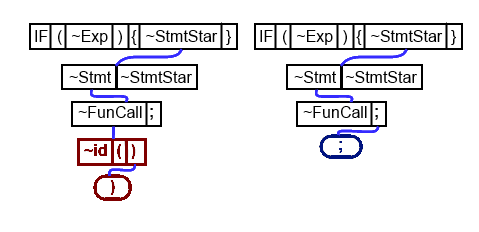
\includegraphics[width=280px]{TokenTraces.png}
\caption{Example of two tokentraces}
\label{fig:traces}
\end{figure}\\
 If at some point there are no possibilities left, but there are still tokens left to be parsed, the compiler will give an error to the user, telling it that their code is uncompilable.
However when a token is allowed, it is mapped to a tokentrace. \textit{(See figure \ref{fig:traces})} A token trace consists of a list of nested expressions, the token that we just parsed and a list of tokentraces that cover the tokens left of this token in the code. So in the right trace in figure \ref{fig:traces}: a funcall inside statement composition inside an if statement, the ";" and the tokentraces that went before this one (which includes the tokentrace on the left). \\
Through this we can get a time-complexity of $\mathcal{O}(n \cdot k) $ with $n$ being the number of tokens in the code, and $k$ being the maximum amount of possible tokens that could follow a certain token. While n can of-course vary per piece of code, $k$ is heavily influenced by how the syntax is written down.\\
Once all tokens of the code have been correctly parsed and the last tokentrace itself doesn't expect a next token, we will have found a correct way of parsing the code. If multiple ways have been found of parsing the same code, this could for example happen when parsing expression only containing a variable, the first possibility is taken, it is up to the structuring of the grammar itself to make sure that this can't lead to two possible parses with differing semantics.
\begin{wrapfigure}{r}{0.35\textwidth}
\centering
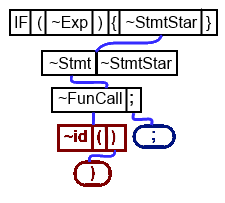
\includegraphics[width=120px]{TokenTree.png}
\caption{Part of a syntaxtree consisting of the two tokentraces described in \ref{fig:traces}}
\label{fig:tracetree}
\end{wrapfigure}
Now that we have a list of tokentraces, the next step is putting them together into a syntax tree.\textit{(See figure \ref{fig:tracetree})}
No errors should be able to occur while the syntax tree is being constructed.\\ 
Once we have constructed the syntax tree, we will convert it into a partially abstract syntax tree. This is done by creating a new ast whilst moving through the tree and checking for each node/expression whether it has an ast equivalent, if it does the equivalent ast node is constructed and added to the new tree, if not a copy of the node is added to the new tree.
\subsection{Expression Optimization}
To reduce time-complexity we parse actual expression separately. Before the above described parsing occurs, the code is first processed, detecting the locations of where an expression should be e.g., when parsing "print 4+5*3;" it will detect the print keyword and then take all tokens between the print keyword and the next ";" i.e. "4+5*3". The extracted tokens are then turned into custom expression tokens, which immediately parse them using the EXP grammar/syntax.
The then parsed expressions are then emmediately checked for any redundant steps, i.e. "4+5*3" will always return 19, thus it is reduced to a simple constant, instead of the more complicated extraction of before.\\
When the actual code is then eventually parsed the syntax just expects an expression token instead of an actual expression.
%expression optimization


\section{Semantic Analysis}
The next step in compiling our code will be semantic analysis. As previously described we've transformed our syntax tree into on with ast nodes.\\
Currently the only semantic analysis that is done, is checking if everything is well-defined and well-typed, and checking whether every non-void function will eventually hit a return statement.\\
\subsection{Type-checking and checking for well-definedness}
Checking if everything is well-typed and well-defined is done in the same step. We do this by traversing the tree and checking the following for each node:
\begin{itemize}
\item Whether the nodes declares anything new e.g., a Variable declaration.
\item Whether the node is well-typed.
\item Whether any undefined id is used.
\end{itemize}
The order in which this is done and how this is done, is entirely dependent and taken care of per node e.g., for a variable declaration it's own name is not allowed to be used in the declaration itself, while in a function declarations body it is allowed to use the function itself such that recursive functions can occur.\\
The ID's that are defined and their types are stored inside of an IDDeclarationblock, this block is then passed through to the next node.
If an id is not declared a declaration exception is thrown. If something is incorrectly typed, for example an integer is assigned to a variable of type boolean, or an expression of type tuple is used in an if-statement, a type exception is thrown.
If an exception is thrown the compiler stops compiling and gives the error to the user.
\subsection{Checking for termination}
Checking whether a non-void function will eventually hit a return statement, is actually already done at the moment its ast node is generated. During generation the function's body is traversed to check, given that it terminates, will eventually hit a return statement. Checking whether the return statement is of the correct type is done later, as described above.

%AST construction
%Monomorphic Type Checking


\section{Code Generation}
\subsection{Basics} %TODO change name?
%call-by-reference
%print only for basic types (otherwise as pointer)
\subsection{Codestack}
%codestack (every node is verantwoordelijk voor zn eigen code)
\subsection{Variables}
%variables
\subsection{Data structures}
%tuples/lists
\subsection{Function calls}
%function calls


\section{Extension}
\subsection{Idea}
%extension idea + motivation
\subsection{Implementation}
%implementation



\appendix
\section{Examples}
%tuple access
%print/isEmpty
%ALL POWERFUL
\end{document}